\documentclass{article}
\usepackage{geometry}
\geometry{margin=.5in}
\usepackage{graphicx} % Required for inserting images
\usepackage{array} % Better table formatting
\usepackage{multirow}
\usepackage[table]{xcolor}
\usepackage{amsmath}
\usepackage{amssymb}
\usepackage[nottoc]{tocbibind}
\usepackage{hyperref}
\usepackage{tikz}
\usepackage{float}
\usepackage{listings}
\usepackage[T1]{fontenc}
\usepackage{inconsolata}
\lstset{
    basicstyle=\ttfamily\footnotesize, % Change font
    breaklines=true,      % Enable line breaking
    breakindent=0pt, %no indent
    breakatwhitespace=false, % Allow line breaks anywhere
    columns=fullflexible, % Ensures proper alignment
    keepspaces=true       % Preserve spaces
}
\usetikzlibrary{positioning}

\title{National Institute of Informatics Internship Report}
\author{Batuhan Karaca}
\date{\today}

\begin{document}
\maketitle
\tableofcontents

\section{Introduction}
I am Batuhan Karaca, a 2nd year MSc student in the University of Freiburg. I was selected for the National Institute of Informatics (NII) internship program for the winter period, 1 October 2024-29 March 2025, to work under Prof. Hideaki Takeda. His main area is \textit{knowledge graphs}.

In the section \textit{Background Research}, the concepts in the related fields, mainly KGs (knowledge graphs) and LLMs (large language models) that are read on are summarized. The tasks are explained in the later sections. Finally, what could have been done better and how the work could be improved in the future is discussed.
\section{Background Research}
The coworkers were PhD students specialized in different areas of KGs. Because I did not have background knowledge in the area, the supervisor first recommended the book "Knowledge Graphs" by Hogan et al. Reading the book took about 1 month. The first part briefly describes the contents of the book. After the book, due to my interest in deep learning and transformer models, the supervisor suggested the paper \textit{Unifying Large Language Models and Knowledge Graphs: A Roadmap} that describes the methods so far in LLM community being used with KGs. I had prior knowledge on transformers due to a deep learning course at the MSc studies. However, I felt the need to polish and expand my knowledge on LLMs in order to understand the concepts in the paper and the future studies. Using the knowledge acquired in BSc, MSc and personal studies, I started to read about the history of LLMs. This process is described in the next part. After feeling ready, I stopped LLM research and started reading the paper, to which the focus is shifted to in the final part. These processes took about 2 weeks.
\subsection{The Book: Knowledge Graphs}
The book starts with a description of different types of a graph, such as a \textit{edge-labeled directed graph}, with a group of nodes where some of the node pairs are connected with one or more edges pointing towards either of the nodes. Each node pair that is connected by an edge is called a \textit{binary relation} or a \textit{triple}. The relations need not be binary, yet they are most of the time for convenience. In this regard, they are similar to a database. Nodes and edges should have an identifier known as \textit{label}. Alongside these labels, another type of graph may include a number of properties for each node and edge, called a \textit{property graph}.

KGs show numerous similarities with a DB (\textit{database}). The stored information could be queried using specific tools such as \textit{SparQL}, a query language similar to SQL. Furthermore, they could have a schema. Relational DBMSs (database management systems) could constrain which group of columns identify a row, the values that the columns could take, and so forth. Given an ontology, there could be multiple ways of describing the same path in a graph that is consistent (or \textit{positive}) with the ontology. A KG (or a DB) with CWA (\textit{closed world assumption}) has no \textit{negative} relations that contradict its constraints, and OWA (\textit{open world assumption}) vice-versa. KGs on the other hand, could govern a much more flexible approach, called \textit{ontology}. Ontologies are a number of logical rules deciding the relationships between the nodes and edges. These paths \textit{entail} and are \textit{entailments} of each other.

Ontologies could be inferred from the graphs using traditional machine learning methods such as rule mining, or rather more novel ones such as NNs (neural networks). Rule mining infers new rules based on the frequency (\textit{confidence}) of the edges in an existing graph. NNs could be trained to output specific ontology features such as class and type; or the aforementioned confidence score. We could then use hidden features of the network for denser representations (\textit{knowledge graph embeddings}) of the graph elements to use for other applications. Recent approaches use transformers such as BERT and LLMs more on which is later. People also tried to create NNs that learn the graphs itself (\textit{graph neural networks}) in the past.

There is another subfield that is interested in constructing the graph from different types of sources as unorganized as plain text, or structured ones such as markup text and tables. When it comes to semantic text, LLMs are preferred compared to methods crafted by hand. The book touches upon how to assess the quality of the constructed graph in terms of metrics. In addition, it points out \textit{refinement} the concept of making the graph consistent with its ontology by adding positive edges (\textit{completion}), and removing negative edges (\textit{correction})\cite{hogan_knowledge_2022}.

\subsection{Reading about LLMs}

\subsubsection{Markov Property and Markov Chain}
Markov property is defined for a stochastic process when the future only depends on the present. The mathematical definition is
\begin{align}
    p(x_t|x_{t-1:0}) &= p(x_t|x_{t-1},x_{t-2},...,x_0)\\
    &= p(x_t|x_{t-1})
\end{align}
where $p$ denotes probabilities. Markov property is a fundamental assumption that facilitates working with temporal data, whether it is the current token of a sentence (natural language processing) or the current state of an environment (reinforcement learning). This assumption seems limiting at the first glance. However, the tokens in the past still indirectly influence the current token. We could also use a running window (e.g. LLM context window) to encapsulate a set of tokens as a compound token \cite{karaca_ai-book_2024}.
\subsubsection{Recursive Neural Networks}
Assuming we have a sequence $x_{1:T} = x_1, x_2, ..., x_T$ a RNN (\textit{Recursive Neural Network}) layer computes
\begin{align}
    h(x_t) &= f\big(\underbrace{h(x_{t-1})w_{(t-1)0} + x_{t-1}w_{(t-1)1} + b_{t-1}}_{g(x_{t-1})}\big)\\
\end{align}
Where $f$ is an activation function. It is easy to see that RNNs have the Markov property. Using the chain rule we have
\begin{align}
    \frac{\delta h(x_t)}{\delta h(x_{t-t_0})}
    &= \prod_{\tau=1}^{t_0}\frac{\delta h(x_{t-\tau+1})}{\delta h(x_{t-\tau})}\\
    &= \prod_{\tau=1}^{t_0}\frac{\delta h(x_{t-\tau+1})}{\delta g(x_{t-\tau})}\frac{\delta g(x_{t-\tau})}{\delta h(x_{t-\tau})}\\
    &= \prod_{\tau=1}^{t_0}f'\Big(g(x_{t-\tau})\Big)w_{(t-\tau)0}
\end{align}
For a stable activation flow, we need
\begin{align}
    f'\Big(g(x_{t-\tau})\Big)w_{(t-\tau)0} &= \pm 1\\
    f\Big(g(x_{t-\tau})\Big) &= \pm \frac{g(x_{t-\tau})}{w_{(t-\tau)0}} + c
\end{align}
where $c$ is a constant w.r.t (with respect to) $g$. $f$ is a linear function w.r.t $g$, unlike $\tanh$ that is used with conventional RNNs. Deep network layers need to have nonlinear components as well. Therefore, Hochreiter et al. decided to use nonlinear activations in the input $g(x_{t-\tau})$ itself. Each nonlinear structure is called a \textit{gate}. This overall layer is called LSTM (long short-term memory) and could be stacked just like a standard RNN layer \cite{hochreiter_long_1997}. Some works stack two inverted RNN layers in order to enable the network to see future tokens as well as the past ones, called BiRNN (bidirectional RNN).

At the time, the NLP (natural language processing) community used a stack of RNN layers that grabs the contextual information out of the input (\textit{encoder}), and another stack of layers that processed this information for the output (\textit{decoder}) for tasks involving sequence transformation (i.e. translation). The current token is accepted at each layer, whereas the decoder layer output is used as the prediction for the next token.

Having different variants, \textit{(cross) attention} between vectors $a, b$ is (with a similarity matrix $S$)

\begin{align}
    S_{ij} &= a_i b_j\\
    A(a,b)_{i} &= \bar{b}_{i} = \sum_j S_{ij} b_j
\end{align}

The attended vector $\bar{b}$ takes into account the similarity between both vectors.

Bahdanau et al. obtain candidate vectors at each layer of a gated BiRNN encoder with a full sweep. Then they use attention between the candidate vectors and the current decoder hidden state to obtain a context vector. Finally, they feed the context vector alongside the current hidden state to obtain the next hidden state for the current gated decoder layer \cite{bahdanau_neural_2016}. ELMo (Embeddings from Language Models, Peters et al.) on the other hand uses deep BiRNNs and concatenates the hidden state vectors. These vectors then could be further concatenated with the input for other NLP tasks \cite{peters_deep_2018}. Parikh et al. and Seo et al. use bidirectional (two-way) cross-attention \cite{parikh_decomposable_2016, seo_bidirectional_2018}.

Lastly, it is important to mention two different training modes for RNNs. When training at the current step, we could feed the current label (correct output) to the network. This is called \textit{teacher forcing} as the name implies. When generating its own output, the network does not have the labels. Teacher forcing resembles spoon learning in an informal sense. There is an alternative called \textit{curriculum learning} that feeds the network its current prediction as the next token. This approach is slower yet achieves better results \cite{lapan_deep_2020}.
\subsubsection{Transformers}
The transformers paper (Vaswani et al.) brought a new paradigm. The first transformer uses an architecture similar to the aforementioned encoder-decoder (\textit{seq2seq}) model. Transformer encoder and decoder blocks process the inputs in parallel unlike RNNs' which operates sequentially. In order to obtain a single output token, the last decoder layer is connected to a FFN (feed forward neural network). The parallelism enables a different attention mechanism at each layer, where the sentence would be compared to itself (self-attention). This allows for faster inference. However, due to its parallel nature, the cross-attention in decoder layers may include future tokens as well. We are not interested in the future tokens that are not available yet, hence the parts corresponding to them are masked \cite{vaswani_attention_2023}.

The transformer boom brought different variants. BERT (Bidirectional Encoder Representations from Transformers, Devlin et al.) is the encoder part of the transformer. It is trained on two tasks. The first task is MLM (masked language modeling) where the network is trained to predict a number of masked tokens for each given sentence. In a typical transformer layer, the future tokens also see the past tokens. In the following layers the current token would indirectly link to itself and the similarity matrix entry corresponding to it would have the highest activation (which is reasonable as it is the same token). Masking the tokens prevents this phenomenon. There is also NSP (next sentence prediction) task where the network is trained to predict the next sentence as the name implies. The authors claim and show, the same \textit{pretrained} network excels at wide range of tasks "such as question answering and language inference" after only little more training, called \textit{fine-tuning} \cite{devlin_bert_2019}. Due to requiring less compute-time, fine-tuning becomes a widely adopted method in the community. GPT (Generative Pretrained Transformer, Radford et al.) on the other hand, uses the decoder part of the transformer \cite{radford_improving_2018}. Three branches (encoder only, decoder only and encoder-decoder) of transformers continue developing.

GPT-3 (Brown et al.) removes the fine-tuning step altogether, proposing \textit{manual few-shot prompting} with hard labels and frozen weights after pretraining \cite{brown_language_2020}. Prompt engineering becomes another paradigm of research. Schickt and Schütze propose \textit{prompt tuning} modelling the problem as a sequence classification task. They fine-tune an ensemble of PLMs (pretrained language models) to predict the relevant masked part, alleviating the contextual information in the prompt given beside the query. Then the PLMs soft-label a larger prompt dataset, giving rise to automatic prompting \cite{schick_exploiting_2021}.

\subsection{The Paper: Unifying Large Language Models and Knowledge Graphs: A Roadmap}\label{kgllm}

The paper divides the approaches into three parts. KG-enhanced LLMs aim to increase accuracy of the answers (i.e. prevent hallucinations) by introducing KGs as structured information to the LLM. LLM-augmented KGs, on the other hand utilizes LLMs in the construction and refinement of KGs. There is another approach called Synergized LLMs + KGs \cite{pan_unifying_2024} to which there was not time to read and understand. I could only read KG-enhanced LLMs.

KG-enhanced LLMs are further divided. Firstly, there are works using KG information in the training objective \cite{pan_unifying_2024}. GLM (Graph Guided Mask LM) uses KGs to mask each entity with a sample. Sampling weight for each entity depends on document frequency and shortest distance to the target entity. They also sample a \textit{negative entity} as they call it. The similarity score between the positive-negative pair is added to the MLM loss to improve generalization \cite{shen_exploiting_2020}. EBERT has a masking method that adaptively switches from words (MLM) to more complex domain relevant phrases. It further uses an association graph to sample neighboring pairs, creating semantic-aware embeddings for each phrase of a pair using cross attention \cite{zhang_e-bert_2021}.

Some methods aim to fuse textual and knowledge information \cite{pan_unifying_2024}. ERNIE adapts the encoder only transformer (i.e. BERT) to the structured knowledge. It stacks a number of textual encoder (T-encoder) layers which do what a typical encoder does with a sentence input. The difference comes with knowledgeable encoder (K-encoder) that comes after it which takes the entities as input. Each K-encoder layer mixes the text-knowledge pair, outputting another text-knowledge pair that are more aware of each other for the next layer \cite{zhang_ernie_2019}. On the other hand, there are methods that include KG information in the input. For instance, ERNIE 3.0 is trained with each relation triple concatenated with its corresponding text as input \cite{sun_ernie_2021}. Some works are prompt-tuning based. KP-PLM approach uses knowledge-aware prompts next to contextual text, then fine-tunes a PLM on this input \cite{wang_knowledge_2022}.

The methods above do not adapt well to the changing data, requiring retraining for the new samples. There is another branch of studies focused on using the knowledge during inference \cite{pan_unifying_2024}. In the REALM paper, Given a context $x$, encoded as dense vectors as query; top scoring encoded document variables $z$ are obtained via MIPS (Maximum Inner Product Search, which works like the attention mechanism) from a KB (knowledge base). Later, $x$ and $z$ are concatenated as input to a generator that is pre-trained on MLM and fine-tuned on open domain QA. The (input and document) encoders and the generator are BERT models. The pipeline is trained end-to-end. For a stable optimization, the document encoder’s parameters are updated periodically \cite{guu_realm_2020}. RAG (retrieval augmented generation) uses an encoder-decoder (seq2seq) transformer (BART) as the generator and fixed document encoders \cite{lewis_retrieval-augmented_2021}. Story fragments adds a short-term memory in which newly seen passages are added. This memory indirectly contributes salience information \cite{wilmot_memory_2021}. EMAT uses MIPS search between a query and a number of keys each mapping to a value in a memory. The obtained key-value pairs are incorporated into the encoder part of a seq2seq transformer \cite{wu_efficient_2022}.
\section{Task: Relation Extraction via Manual Prompting}\label{relx_manual_prompt}
The supervisor suggested a simple idea. I was expected to have an LLM model output triples for a given passage via prompt engineering. The LLM was going to process the prompt without intermediary steps during inference. I started searching along the lines of \texttt{graph construction via prompting}, expecting to find abundant materials. The works that are found if any, either had prompts that are not suitable for task, or were using complex approaches that are not end-to-end. Most of the works are only skimmed through. One of such works is by Carta et al. which uses multiple steps (as the name "iterative" in the title) \cite{carta_iterative_2023}. The scarcity of the results was probably due to the terms given to the search engine. I could have been more descriptive or used different words. In the last month of the internship period, replacing the phrase \texttt{graph construction} with its formal counterpart \textit{relation extraction} in the search term, resulted in more promising results. I was not familiar with the term \textit{relation extraction} at the start of the internship. Results were not checked due to limited time.

Query part of the most promising prompt that Zhu et al. is used with some modifications. With their prompt Zhu et al. claim to achieve a micro-F1 score of 4.4 and 7.2 using ChatGPT web interface and the GPT-4 model on SciERC dataset respectively. However, they do not describe whether they fine-tuned GPT-4 and which model they used for the ChatGPT and so forth \cite{zhu_llms_2024}. The prompts and their results are given in part~\ref{man_prompts}. List of predicates could grow with number of edge classes a KG has. This could be a problem when \textit{context window} (maximum number of tokens input has) of an LLM is smaller than the prompt, though this never happened with the models that are tried. Nevertheless, another version of the prompt which does not have the list of predicates is also used in the experiment.

Before proceeding, there are problems to point out on accuracy of the outputs. Firstly, it is challenging to find a suitable ground truth. Due to the constrained nature (i.e. schema and ontology) of KGs, the number of classes that the nodes and edges could take is finite. Assuming CWA, if a KG represents the real world accurately (without any negatives in the real world data that the LLM is trained on), it could be used as a ground truth for evaluation. Secondly, the LLM may give a set of outputs that entail a set of triples in the label set. In this case, the KG is accurate yet the LLM performs worse as these outputs are not true-positive. In other words, an LLM output could either be negative or positive, yet not in the label set. For brevity, CWA is assumed, excluding the problematic positive outputs from true-positives. Lastly, the \textit{power} or how accurately the LLM represents the ground truth is important as well. The number of parameters is one of the factors that influence this variable to some extent. The LLMs with higher number of parameters generally tend to be more powerful (perform better).

Few inputs with 0, 1 and 2-shot prompts are tested. A prompt may differ due to its number of \textit{demonstrations} where each demonstration is an input-label pair, similar to a supervised setting. An N-shot prompt uses N demonstrations. The query input is given at the end. TACRED dataset is preferred as the ground truth which has plenty of competition entries for F1 score evaluation \cite{zhang_position-aware_2017,noauthor_tacred_nodate}. It still has some inherent problems as well, discussed in detail in Re-TACRED paper \cite{stoica_re-tacred_2021}. ChatGPT free plan (which used the GPT-4o at the time) and Phi-3 mini are used. The authors show that with only 3.8 billion parameters, Phi-3 mini performs close (or sometimes better) compared to models as large as 7 billion parameters. The variant with smaller context window of 4000 tokens is used (there is also a variant with 128000) \cite{abdin_phi-3_2024}. Calculating the token length for the prompts, the maximum value was 668, making larger context windows unnecessary due to memory concerns.

Without the list of predicates, the models were creating their own \textit{explicit} relations. For such a triple, they either came up with a verb in the sentence as predicate; or a paraphrase of the verb. Adding the list of predicates to constrain the model did not prevent models from outputting irrational outputs as well. For instance, ChatGPT outputted predicate values where they should not be (i.e. in place of tail values). Phi-3-mini performed worse. For some of the prompts, it did not comply with the prompts (i.e. plain Python list), giving outputs in different formats (e.g. markup languages, numbered list). Because Phi-3 is a family of open-source models, it is possible to adjust their generation parameters such as \textit{temperature}. $\text{Temperature}=0$ as suggested in the paper without sampling (i.e. greedy search). The generation parameters could have been manually fine-tuned. However, I decided to see if automatic fine-tuning is possible. There are existing hyperparameter tuning methods for cross-validation which seemed tricky to implement for manual prompting.

\section{Task: Prompt Tuning via Light-weight LLM}

Due to the problems in the previous part, another idea was conceived. A lightweight LLM was going to be fine-tuned on a set of sentence-triple pairs, then the model performance was going to be evaluated. Separate model wasn't needed for prompt generation. Only a single model would be trained end-to-end, bearing the name \textit{end-to-end prompt tuning} for the project. Good enough fine-tuning could make a lightweight model more powerful. The scale of the model could be a plus for individual applications.

It is possible to train a NN using plain supervised learning. However, I did not want to stop here and wanted to experiment with different training methods. There is a ton, yet starting simple would be more preferable. LLMs and RL methods are known to have Markov property. I decided to read on RL. I was looking for a book that also included implementations with the theory, so I came across \textit{Deep Reinforcement Learning Hands On} by Maxim Lapan. I read the book until the end of \textit{Chapter 14: Training Chatbots with RL} which took about 2 weeks. The implementation is based on seq2seq RNNs which is adapted to a decoder only LLM in the task. After Deepseek-R1 came out, its authors claimed that they were also using a similar technique to train their model. The technique is a \textit{policy gradient method}, called GRPO (\textit{Group
Relative Policy Optimization}) \cite{deepseek-ai_deepseek-r1_2025, shao_deepseekmath_2024, schulman_proximal_2017}. \textit{REINFORCE} which is one of the least sophisticated methods to implement in this family is adopted. At the time, the implementation was already ready and reimplementing GRPO seemed risky.

In the upcoming two parts, the concepts from the book and other resources that are relevant to the task are explained. In the final two parts, the metrics used during training and evaluation, with the implementation details at the end are described.
\subsection{Reinforcement Learning Concepts}
RL agent acts on a tuple $(s_t,r_t)$ at time step $t$ where $s_t$ is the current state and $r_t$ is the reward resulting from $s_t$. Each action $a_t$ taken by the agent results in another tuple at time step $t+1$. It is easy to see that this has the Markov property.

For any initial state $s_t$, the cumulative reward is defined as
\begin{align}
    g_t &= \lim_{N\rightarrow\infty}\sum_{\tau=0}^N \gamma^\tau r_{t+\tau}\\
    \sum_{\tau=0}^N \gamma^\tau r_{\min} &\leq\sum_{\tau=0}^N \gamma^\tau r_{t+\tau}\leq\sum_{\tau=0}^N \gamma^\tau r_{\max}\\
    \frac{\gamma^{N+1}-1}{\gamma-1}r_{\min} &\leq\sum_{\tau=0}^N \gamma^\tau r_{t+\tau}\leq\frac{\gamma^{N+1}-1}{\gamma-1}r_{\max}\\
    \lim_{N\rightarrow\infty}\frac{\gamma^{N+1}-1}{\gamma-1}r_{\min} &\leq\lim_{N\rightarrow\infty}\sum_{\tau=0}^N \gamma^\tau r_{t+\tau}\leq\lim_{N\rightarrow\infty}\frac{\gamma^{N+1}-1}{\gamma-1}r_{\max}\\
    \frac{r_{\min}}{1-\gamma} &\leq g_t\leq\frac{r_{\max}}{1-\gamma}\ \scriptstyle{\text{if $0 \leq \gamma < 1$}}
\end{align}
As long as the rewards are bounded and $0 \leq \gamma < 1$, the cumulative reward will always be bounded as well, which is preferred. Getting diminishing returns as a result prevents the agent to go for infinite loops for infinite gain, encouraging to finish as soon as possible.
\subsubsection{Bellman Equation}
\begin{align}
    V(s_t)
    &= \sum_{g_t}p\big(g_t|s_t\big)g_t\\
    &= E\big(g_t|s_t\big)\\
    &= E\big(r_{t}+\gamma g_{t+1}|s_t\big)\\
    &= E(r_t|s_t)+\gamma E\big(g_{t+1}|s_t\big)\\
    &= \sum_{r_t}p\big(r_t|s_t\big)r_t+\gamma \sum_{g_{t+1}}p\big(g_{t+1}|s_t\big)g_{t+1}\\
    &= \sum_{r_t,a_t,s_{t+1}}p\big(r_t,a_t,s_{t+1}|s_t\big)r_t+\gamma \sum_{g_{t+1}}\sum_{r_t,a_t,s_{t+1}}p\big(g_{t+1}|r_t,a_t,s_{t+1},s_t\big)p\big(r_t,a_t,s_{t+1}|s_t\big)g_{t+1}\\
    &= \sum_{r_t,a_t,s_{t+1}}p\big(r_t,a_t,s_{t+1}|s_t\big)\left[r_t+\gamma \sum_{g_{t+1}}p\big(g_{t+1}|r_t,a_t,s_{t+1},s_t\big)g_{t+1}\right]\\
    &= \sum_{r_t,a_t,s_{t+1}}p\big(r_t,a_t,s_{t+1}|s_t\big)\left[r_t+\gamma \sum_{g_{t+1}}p\big(g_{t+1}|s_{t+1}\big)g_{t+1}\right]\\
    &= \sum_{r_t,a_t,s_{t+1}}p\big(a_t|s_t\big)p\big(r_t,s_{t+1}|a_t,s_t\big)\big[r_t+\gamma V(s_{t+1})\big]\\
    &= \sum_{a_t}p\big(a_t|s_t\big)\sum_{r_t,s_{t+1}}p\big(r_t,s_{t+1}|a_t,s_t\big)\big[r_t+\gamma V(s_{t+1})\big]\\
    &= \sum_{a_t}\pi\big(a_t|s_t\big)Q(a_t, s_t)\\
    V(s_t) &= E_\pi\big[Q(a_t, s_t)\big]\\
    Q(a_t, s_t) &= E_{r_t, s_{t+1}}\big[r_t+\gamma V(s_{t+1})\big]\label{valueexp}
\end{align}
$V, Q, \pi$ are called \textit{value function}, \textit{Q-function} and \textit{policy} respectively.
\subsubsection{Value Based Methods}
\textit{Value based methods} assume a fixed policy (i.e. choosing the maximum value). In the expression~\ref{valueexp}, when we fix the policy such that the possibility of the maximum value is 1 we have
\begin{equation}
    V^*(s_t) = \max_{a_t}\big[Q(a_t, s_t)\big]
\end{equation}

Alternatively, we could visualize this phenomenon as a graph in figures~\ref{fig:rl_graph} and~\ref{fig:rl_tree}. The agent maximizes the reward by climbing the tree in figure~\ref{fig:rl_tree} in a maximin fashion. For real life scenarios construction the tree could be costly. Therefore, people generally prefer using sampling methods such as Monte Carlo.

% Graph figure
\begin{figure}[H]
\centering
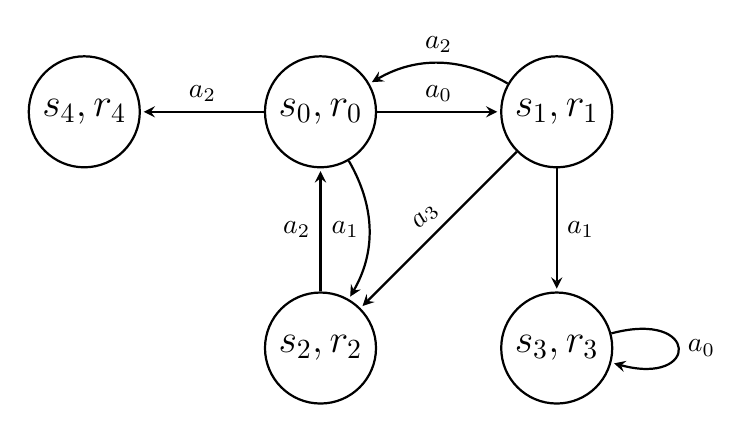
\begin{tikzpicture}[->, >=stealth, shorten >=1pt, auto, node distance=3cm, thick, main node/.style={circle, draw, font=\sffamily\Large\bfseries}]

  % Define nodes
  \node[main node] (s0) {$s_0, r_0$};
  \node[main node] (s1) [right of=s0] {$s_1, r_1$};
  \node[main node] (s2) [below of=s0] {$s_2, r_2$};
  \node[main node] (s3) [below of=s1] {$s_3, r_3$};
  \node[main node] (s4) [left of=s0] {$s_4, r_4$};

  % Define edges with labels (including new s1->s2 edge)
  \path[->]
    (s0) edge node[above] {$a_0$} (s1)
    (s1) edge node[right] {$a_1$} (s3)
    (s2) edge node[left] {$a_2$} (s0)
    (s3) edge[loop right] node[right] {$a_0$} (s3)
    (s0) edge[bend left] node[left] {$a_1$} (s2)
    (s1) edge[bend right] node[above] {$a_2$} (s0)
    (s1) edge node[sloped, above] {$a_3$} (s2)
    (s0) edge node[above] {$a_2$} (s4);
\end{tikzpicture}
\caption{A sample graph of a state space}
\label{fig:rl_graph}
\end{figure}

% Tree figure
\begin{figure}[H]
\centering
\resizebox{.5\textwidth}{!}{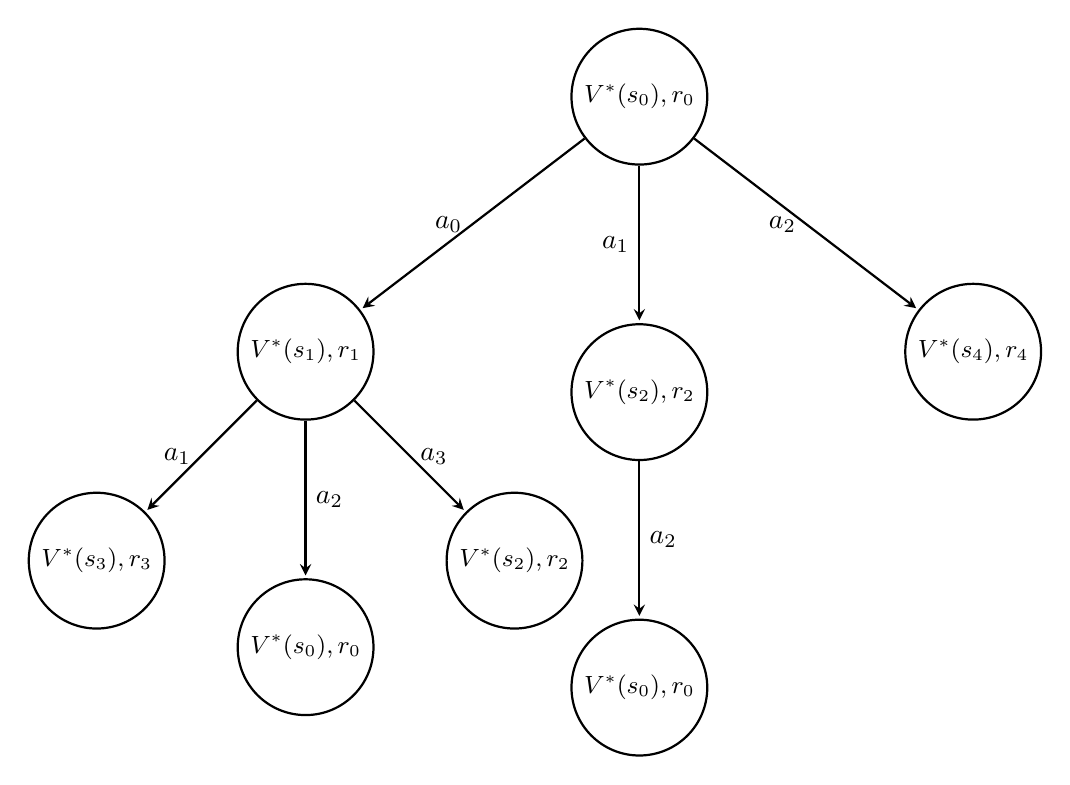
\begin{tikzpicture}[->, >=stealth, shorten >=1pt, auto, node distance=2cm, thick,
    main node/.style={circle, draw, align=center, font=\small}]

  % Nodes (arranged top-to-bottom)
  \node[main node] (s0) {$V^*(s_0), r_0$};

  % Level 1
  \node[main node] (s1) [below left=2cm and 3cm of s0] {$V^*(s_1), r_1$};
  \node[main node] (s2) [below=2cm of s0] {$V^*(s_2), r_2$};
  \node[main node] (s4) [below right=2cm and 3cm of s0] {$V^*(s_4), r_4$};

  % Level 2 (from s1)
  \node[main node] (s3) [below left=of s1] {$V^*(s_3), r_3$};
  \node[main node] (s0a) [below=of s1] {$V^*(s_0), r_0$};
  \node[main node] (s2a) [below right=of s1] {$V^*(s_2), r_2$}; % New node

  % Level 2 (from s2)
  \node[main node] (s0b) [below=of s2] {$V^*(s_0), r_0$};

  % Edges with labels (including new path)
  \path[->]
    (s0) edge node[midway, left] {$a_0$} (s1)
    (s0) edge node[midway, left] {$a_1$} (s2)
    (s0) edge node[midway, left] {$a_2$} (s4)
    (s1) edge node[midway, left] {$a_1$} (s3)
    (s1) edge node[midway, right] {$a_2$} (s0a)
    (s1) edge node[midway, right] {$a_3$} (s2a) % New edge
    (s2) edge node[midway, right] {$a_2$} (s0b);
\end{tikzpicture}}
\caption{Tree of all paths in the graph in figure~\ref{fig:rl_graph} with length less than or equal to 2}
\label{fig:rl_tree}
\end{figure}
\subsubsection{Policy Gradient Methods}
There is another branch of methods called \textit{policy gradient methods} that uses gradient to adapt a model to a dynamic policy \cite{lapan_deep_2020}. The accumulated reward independent of a state could be expressed as below
\begin{align}
    J(\theta)
&= \sum_{s \in \mathcal{S}} d^\pi(s) V^\pi(s) \\
&= \sum_{s \in \mathcal{S}} d^\pi(s) \sum_{a \in \mathcal{A}} \pi_\theta(a \vert s) Q^\pi(s, a)\\
&= \sum_{s \in \mathcal{S}} d^\pi(s)\sum_{a \in \mathcal{A}} \pi_\theta(a \vert s) \sum_{s'} P(s' \vert s,a) \nabla_\theta V^\pi(s')
\end{align}
Analytically calculating the gradient is tricky. Only policy is parameterized; however, the value terms include the policy as well. Following the derivation in Lilian Weng's blog gives (please refer to the blog for full derivation).
\begin{align}
\nabla_\theta J(\theta)
&= \nabla_\theta \sum_{s \in \mathcal{S}} d^\pi(s) \sum_{a \in \mathcal{A}} Q^\pi(s, a) \pi_\theta(a \vert s) \\
&\propto \sum_{s \in \mathcal{S}} d^\pi(s) \sum_{a \in \mathcal{A}} Q^\pi(s, a) \nabla_\theta \pi_\theta(a \vert s) \\
&= \sum_{s \in \mathcal{S}} d^\pi(s) \sum_{a \in \mathcal{A}} \pi_\theta(a \vert s) Q^\pi(s, a) \frac{\nabla_\theta \pi_\theta(a \vert s)}{\pi_\theta(a \vert s)} \\
&= \mathbb{E}_\pi \big[Q^\pi(s, a) \nabla_\theta \ln \pi_\theta(a \vert s)\big]\ \scriptstyle{\text{because } (\ln x)' = 1/x} \label{policy_grad}
\end{align}
One policy gradient method (maybe the simplest) is \textit{REINFORCE}, given as below.
\begin{enumerate}
    \item Predict the reward $G_t$
    \item Perform a gradient update $\theta \leftarrow \theta + \alpha \gamma^t G_t \nabla_\theta \ln \pi_\theta(A_t \vert S_t)$\ \cite{weng_policy_2018}
\end{enumerate}
During the mean loss calculation, sample mean of the accumulated gradients are calculated. This gives an approximation for~\ref{policy_grad}, in a Monte Carlo manner. As the predicted reward values may have high variance they lead to unstable optimization. For smoother gradient updates, the coefficient term is generally normalized with a \textit{baseline} as $Q(a,s)-b(s)$. For a baseline, the mean $V(s) = E_a[Q(a,s)]$ could be used. The book uses the optimal value $V^*(s) = \max_a[Q(a,s)]$ from the SCST (\textit{self-critical sequence training}) paper \cite{lapan_deep_2020, rennie_self-critical_2017}. It is possible to use a NN to approximate the rewards as well, which is done with methods such as \textit{actor-critic}. The book's implementation uses BLEU metric as the reward estimation \cite{lapan_deep_2020}.
\subsection{LoRA (Low-Rank Adaptation of Large Language Models)}\label{lora}
When training NNs, the parameters and gradients could be sparse. Their matrix representation could be rewritten as sum of products of matrices with smaller ranks as below.
\begin{equation}
    W = \sum_i A_iB_i
\end{equation}
Hu et al. choose to approximate the gradient of a layer with a single product. The product could be modeled as a forward pass of two smaller layers called \textit{adapters}. In previous works, the adapters were injected between the original parameters. However, Hu et al. train the adapters alongside the parameters. This ensures the network depth stays the same, reducing the number of sequential operations allowing for faster inference. The expression for a composite linear-LoRA layer structure is given below.
\begin{equation}
    h = (W + \Delta W)x = (W + \gamma_rAB)x
\end{equation}
Instead of large number of network parameters, adapter parameters correspond to only a small portion of these parameters. The adapters could be removed and attached. In this regard, LoRA is a modular and lightweight approach. The authors also use a coefficient $\gamma_r=\frac{\alpha}{r}$. Tuning $\alpha$ is not important as it corresponds to roughly the learning rate when optimizing with Adam \cite{hu_lora_2021}. The authors divide by the rank $r$ as the dot product term becomes larger with larger ranks.
\subsubsection{RS-LoRA (Rank-Stabilized LoRA)}
RS-LoRA paper shows that for a network with $m$ layers, after $n$ gradient updates, the complexities for the expressions of forward pass output and gradients are $\Theta_r((\gamma^2_rr)^m)$ and $\Theta_r(\gamma^2_rr)$ respectively. The vanilla coefficient results in diminishing values (i.e. $\Theta_r\big(\frac{1}{r^m}\big)$ and $\Theta_r\big(\frac{1}{r}\big)$), leading to instability and worse performance. Instead, RSLoRA uses $\gamma_r = \frac{\alpha}{\sqrt{r}}$ for stability (i.e. $\Theta_r(1)$) \cite{kalajdzievski_rank_2023}.
\subsubsection{Q-LoRA(Quantized LoRA)}\label{qlora}
Differentiation libraries (e.g. autograd of PyTorch) use intermediary variables such as the gradients for their calculations. We roughly need double the size of the model itself only to store gradients. Q-LoRA quantizes the stored parameters to 4-bit, as NF-4 (\textit{NormalFloat}) type. During forward/backward pass, the parameters of the computed layer are dequantized to 16-bit, as bfloat (\textit{BrainFloat}) type \cite{dettmers_qlora_2023}. Bfloat maps to the same range with 32-bit representation with less precision as shown in figure~\ref{fig:bfloat} to prevent overflow errors. NF4 uses a lookup table of 16 \textit{q-values} in the range [-1, 1], index of which is the stored 4-bit value. As long as the weights are normally distributed, NF4 equally distributes the q-values  as illustrated in figure~\ref{fig:nf4} \cite{dettmers_8-bit_2022}.

\begin{figure}[H]
    \centering
    \includegraphics[width=0.5\linewidth]{pictures/bfloat.png}
    \caption{Depiction of three floating point representations in memory \cite{grobbelaar_pygmalionaipygmalion-7b_2023}}
    \label{fig:bfloat}
\end{figure}

\begin{figure}[H]
    \centering
    \includegraphics[width=0.5\linewidth]{pictures/nf4.png}
    \caption{Gaussian PDF and CDF plot from top to bottom in the Interval $[-1, 1]$ with q values}
    \label{fig:nf4}
\end{figure}
\subsubsection{LoftQ (LoRA-Fine-Tuning-aware Quantization)}
LoRA initializes $A$ with a normal distribution, and $B=0$. LoftQ aims to find an initialization such that the inference error is minimized. It achieves it by using an iterative approach.
\begin{align}
    Wx &= (Q+AB^T)x\\
    (W-Q-AB^T)x &= 0\\
    \lVert W-Q-AB^T\rVert &= 0
\end{align}
Where $\vert\vert$ denotes the matrix norm we are trying to minimize \cite{li_loftq_2023}.
\subsection{Metrics}
\subsubsection{Evaluation Metric: F1 score}
For any task, one could form a confusion matrix by saving the actual and predicted values as in figure~\ref{fig:confusion_matrix}. A target class $c$ could have set of  \textit{true positives},  \textit{true negatives},  \textit{false positives} and  \textit{false negatives} with cardinalities $TP_c$, $TN_c$, $FP_c$ and $FN_c$ respectively as shown in the figure. Note that we are interested in multiple classes.

\begin{figure}[H]
\centering
\renewcommand{\arraystretch}{1.5} % Increase row height for better readability
\begin{tabular}{c|c|c|c|c|c|c|}
 \multicolumn{2}{c}{} & \multicolumn{5}{c}{\textbf{Predicted values}} \\ \cline{3-7}
\multicolumn{1}{c}{} & & A & B & C & D & E \\ \cline{2-7}
\multirow{5}{*}{\rotatebox{90}{\textbf{Actual values}}} & A & \cellcolor{green!25} 3 & \cellcolor{red!25} 7 & 2 & 9 & 5 \\ \cline{2-7}
& B & \cellcolor{yellow!50} 6 & \cellcolor{blue!25} 1 & \cellcolor{yellow!50} 8 & \cellcolor{yellow!50} 4 & \cellcolor{yellow!50} 2 \\ \cline{2-7}
& C & 9 & \cellcolor{red!25} 5 & \cellcolor{green!25} 3 & 7 & 6 \\ \cline{2-7}
& D & 4 & \cellcolor{red!25} 8 & 1 & \cellcolor{green!25} 2 & 9 \\ \cline{2-7}
& E & 7 & \cellcolor{red!25} 3 & 6 & 5 & \cellcolor{green!25} 4 \\ \cline{2-7}
\end{tabular}
\caption{A sample confusion matrix of 5 classes. The areas colored blue, green, red and yellow sum up to $TP_B$, $TN_B$, $FP_B$ and $FN_B$ respectively}
\label{fig:confusion_matrix}
\end{figure}

\textit{Precision} and \textit{recall} are defined as
\begin{align}
    \text{precision}_c &= \frac{TP_c}{TP_c + FP_c} = \frac{TP_c}{\text{number of predictions for $c$}} \label{prec}\\
    \text{recall}_c &= \frac{TP_c}{TP_c + FN_c} = \frac{TP_c}{\text{number of instances for $c$}} \label{recall}\\
\end{align}
\textit{F1 score} incorporates both these values via harmonic sum.
\begin{equation}
    \text{F1 score}_c = \frac{2}{\frac{1}{\text{precision}_c} + \frac{1}{\text{recall}_c}}
\end{equation}
Macro and micro F1 scores are defined as follows \cite{leung_micro_2022}.
\begin{equation}
    \text{F1 score}_\text{macro} = \frac{1}{C}\sum_c \text{F1 score}_c\ \scriptstyle{\text{where $C$ is the number of classes}}
\end{equation}
We define $TP = \sum_c TP_c$ and similarly for other values as well.
\begin{align}
    \text{F1 score}_\text{micro}
    &= \frac{2}{\frac{1}{\text{precision}_\text{micro}} + \frac{1}{\text{recall}_\text{micro}}}\\
    &= \frac{2}{\frac{TP+FP}{TP} + \frac{TP+FN}{TP}}\\
    &= \frac{2}{\frac{2TP+FN+FP}{TP}}\\
    &= \frac{2TP}{2TP+FN+FP}\\
    &= \frac{TP}{TP+\frac{1}{2}(FN+FP)}\\
    &= \frac{TP}{TP+FP} = \text{precision}_\text{micro}\\
    &= \frac{TP}{TP+FN} = \text{recall}_\text{micro}\ \scriptstyle{\text{since $FN=FP$}}\\
    &= \frac{TP}{\text{number of total instances}}\\
    &= \text{accuracy}
\end{align}
\subsubsection{Reward Metrics}
\paragraph{BLEU (Bilingual Evaluation Understudy)}
is a method introduced for MT (machine translation) tasks to assess similarity of two sequences, namely the predicted \textit{candidate} and the ground truth \textit{reference}. Similar to convolution operation, a window capturing a subsequence of n tokens (i.e. \textit{n-gram}) is slid over the sequence. Then the intersecting n-grams form the set of true positives. As in expression~\ref{prec}, dividing by total number of candidate n-grams gives the precision for n, $g_n$ which we call \textit{n-gram score}. Intuitively, duplicate n-grams should not contribute to the score. To alleviate this, number of duplicate matches are clipped with a value (usually 1). This is done only when calculating TP (not the total predictions) in order to penalize duplicate predictions. A candidate sequence could also be compared against multiple references as well (there could be multiple translations giving the same meaning). To give an aggregated similarity metric for multiple references, the total TP is used. Calculating similarity score of a candidate sequence (i.e. passage of text) composed of multiple subsequences (i.e. sentences) separated by a specific token (i.e. dot) is also straightforward. The total TP over the subsequences is divided by the total number of n-grams.

The n-gram scores could be weighted over different $n$ values to give an overall n-gram score as below.

\begin{align}
    G_N &= \prod_{n=1}^{N}g_n^{w_n}\\
    \log G_N &= \sum_{n=1}^{N}w_n\log g_n
\end{align}

We want the candidates to have lengths as close as possible to the references. N-gram score already penalizes the longer predictions. For shorter predictions, we use \textit{brevity penalty} as below
\begin{equation}
    BP = \begin{cases}
        1 & \text{if } c > r\\
        e^{1-\frac{r}{c}} & \text{if } c \leq r
    \end{cases}
\end{equation}
where $c$ refers to the total length of all candidates. $r$ denotes the total reference length. For each candidate the closest reference length is chosen, and the chosen lengths are summed over the candidates, which gives \textit{effective reference corpus length} $r$.

BLEU score is defined as
\begin{align}
    \text{BLEU}_N &= BP\cdot G_N\\
    \log\text{BLEU}_N &= \min(1-\frac{r}{c},0)+\sum_{n=1}^{N}w_n\log g_n
\end{align}
Usually $N=4$ is used as introduced in the original paper \cite{papineni_bleu_2002}.
\paragraph{ROUGE (Recall-Oriented Understudy for
Gisting Evaluation)}
is an umbrella term for a set of approaches. ROUGE-N calculates an n-gram score between a candidate-reference pair similar to BLEU where $N$ is an integer denoting the length of the n-gram. When aggregating n-gram scores over multiple references, it only chooses the maximum scoring reference instead of summing as BLEU does.
\begin{equation}
    \text{ROUGE-N} = \arg_r\max g_n(c,r)\ \scriptstyle{\text{where $(c,r)$ is a candidate-reference pair}}
\end{equation}
ROUGE-L uses LCS (\textit{longest common subsequence}) length between two sentences as TP. Plain ROUGE-L only considers a single LCS. There is another variant $\text{ROUGE-L}_{\text{sum}}$ that takes the union of LCSs for each reference, summing up the union lengths to obtain TP.

ROUGE methods could use recall and F1 scores as the metric unlike BLEU, which only uses precision. ROUGE has other variants as well such as weighted ROUGE-L and ROUGE-S that uses strided n-grams \cite{lin_rouge_2004}. These methods are not described here as they are not used in the task.
\subsection{Implementation}
\subsubsection{Dataset}
A modified version of the prompt in part~\ref{relx_manual_prompt} is used
\begin{quote}
    \texttt{List of predicates is ['org:founded', 'org:subsidiaries', 'per:date\_of\_birth', 'per:cause\_of\_death', 'per:age', 'per:stateorprovince\_of\_birth', 'per:countries\_of\_residence', 'per:country\_of\_birth', 'per:stateorprovinces\_of\_residence', 'org:website', 'per:cities\_of\_residence', 'per:parents', 'per:employee\_of', 'NA', 'per:city\_of\_birth', 'org:parents', 'org:political/religious\_affiliation', 'per:schools\_attended', 'per:country\_of\_death', 'per:children', 'org:top\_members/employees', 'per:date\_of\_death', 'org:members', 'org:alternate\_names', 'per:religion', 'org:member\_of', 'org:city\_of\_headquarters', 'per:origin', 'org:shareholders', 'per:charges', 'per:title', 'org:number\_of\_employees/members', 'org:dissolved', 'org:country\_of\_headquarters', 'per:alternate\_names', 'per:siblings', 'org:stateorprovince\_of\_headquarters', 'per:spouse', 'per:other\_family', 'per:city\_of\_death', 'per:stateorprovince\_of\_death', 'org:founded\_by']. What Subject-Predicate-Object triples are included in the following sentence?}
\end{quote}
List of predicates is included for more degrees of freedom. This allows giving different list of predicates for other graphs.

Preprocessing of the dataset is shown in part~\ref{dataset_transform}. Firstly, the dataset is mapped so that there is only two columns (sentence and labels, sample 1). Then ChatML (\textit{Chat Markup Language}, introduced by OpenAI) template is applied to the dataset (samples 2 and 3). The final step is the tokenization, which is not shown. When training, the triples are injected into the input sequence for reference. However, the model is expected to generate the data during evaluation. The triple is extracted as a separate column to compare the output at this stage. Because model is trained to give its answer after the generation prompt (<|assistant|>), it gives outputs irrelevant to the prompt without it at the end. This occurs during generation, which occurs during evaluation.
\subsubsection{Model and Training}
Web APIs are not preferred as the task requires sending costly bulks of data. Therefore, closed-source GPT variants and alike are avoided. Google Colab is used with occasional switches to Kaggle Notebook. With these tools, access to a compute power to host a large LLM is not possible. Therefore, lightweight LLMs with fewer number of parameters are preferred. Microsoft's Phi, Google's Gemma, Facebook's Llamma are a few. For comparison, GPT-3 has about 175 billion parameters requiring 350GB \cite{brown_language_2020} and is possibly not larger than GPT-4, whereas Phi-3-mini only has 3.8 billion parameters \cite{abdin_phi-3_2024} (2GB memory requirement according to the output of a program written for the work). Phi-3-mini is chosen due to the reasons in part~\ref{relx_manual_prompt}. Due to the memory concerns pointed out in part~\ref{qlora}, lightweight models become extra important for training. PyTorch library enables one to disable unnecessary computations such as gradient calculations and achieve significant memory gain during evaluation. As a side note, the codebase was built around Phi-3-mini. Therefore it was not cost effective to have models such as Phi-4 and Deepseek-R1 work seamlessly. These models were released toward the end of the internship period.

HuggingFace's \texttt{transformers} and \texttt{bitsandbytes} libraries for the model and Q-LoRA implementations are used respectively. Aside the parameters discussed in part~\ref{qlora}, the configuration class also takes the maximum sequence length which is 4096 (the context window size). Flash attention implementation could not be enabled for performance gain. Flash attention supports Ampere, Ada, or Hopper GPUs \cite{dao-ailab_github_2022}. Google Colab offers T4 which is Tesla; therefore, the plain implementation is preferred.

At the beginning, I attempted to use \texttt{Trainer} API of the \texttt{transformers} library. Due to encountered errors, a complete trainer API was written from scratch, which was a bad decision.

The training mostly occurs in the loss function. The model has little information before the training. As training progresses, the model becomes \textit{wiser} (i.e. As it is introduced to more samples, it \textit{knows} more). Therefore, the book's implementation starts with teacher forcing (i.e. label is inputted as the next token), gradually transitioning to curriculum learning (i.e. predicted output is inputted as the next token). Transformers process the inputs in parallel, not allowing the use of curriculum learning. Teacher forcing is preferred during training \cite{lapan_deep_2020}.

The difference between a number (which is a HP) of sampled logits from the model's output distribution and the maximum logit (as the baseline) gives the reward value. The book only considers BLEU as the reward metric \cite{lapan_deep_2020}. BLEU and ROUGE as HPs (hyperparameters) are used for comparison. Default parameters for both are used. For ROUGE, F1 scores of $\text{ROUGE-1}, \text{ROUGE-2}, \text{ROUGE-L}$ and $\text{ROUGE-L}_{\text{sum}}$ are tuned. There are also other metrics such as METEOR that are not used. Due to the fact that TACRED gives a single reference without a separation token, the one-to-one single sequence variants of these metrics are used. There is also the \textit{multiple} (another HP) variant that is built that compares a candidate against all references in the batch. CE (\textit{Cross Entropy}) is used as usual for supervised learning.

The loss function supports \textit{label smoothing}, which is a regularization technique that adds noise to the loss value. The returned loss is a linear interpolation between the original loss and the mean loss to make model decisions less certain for better generalization \cite{muller_when_2020}. The interpolation constant \textit{label smoothing factor} is another HP.

For the LoRA parameters, Tuning $\alpha$ is unnecessary as mentioned in~\ref{lora}. Only the rank $r$ is tuned. The value closest to exponential median is used (The range is $r \in [1=2^0, 64=2^6]$ with median $8=2^3$, $32$ is chosen). LoRA adapters are type of NNs that could use regularization techniques. Therefore, they support dropout regularization, which is another HP. Even though LoftQ is described in the report, it is very challenging to use it. It is an iterative LoRA initialization method with complexity proportional to the number of adapter parameters. Because NNs tend to be more powerful with higher number of parameters, LoRA adapters are injected to all linear layers. Therefore, it took considerable time to compute LoftQ initialization. For each different LoRA rank, the parameters had to be reinitialized. There are precomputed LoftQ adapters available on the internet for some LoRA configurations, which is not matching the specified configurations of the task. RS-LoRA is used as well.

Lastly, \textit{AdamW} is used for the optimizer \cite{loshchilov_decoupled_2019}. The learning rate, betas, and weight decay are tuned.
\subsubsection{Evaluation}
The papers in part~\ref{relx_manual_prompt} were using F1 score. Micro F1 is used for evaluation. A unique triple is considered as a class. Instead of a CxC confusion matrix ($O(C^2)$), a counter of classes ($O(C)$) is constructed. The memory gain from this approach could be beneficial for larger KGs. For each prediction-label pair, the intersection gives true positives. The total number of true positives and the total length of both predictions and labels are used in the calculation.

There are multiple ways to generate an output in a sequential manner. Greedy search chooses the token with the maximum value. Beam search with a number of beams $B$ expands for the top $B$ scoring tokens at each level, decrementing $B$ by 1. Deterministic techniques such as these could lead to repetitive outputs. The tokens could be sampled from the distribution. Alternatively, values below a certain probability threshold $p$ could be eliminated \cite{holtzman_curious_2020}. A number of values in the API (\texttt{do\_sample}, \texttt{num\_beams}, \texttt{top\_p}) are tuned to compare between such techniques. Lastly, temperature works similarly to label smoothing factor, preventing the network from going too certain.
\subsection{Hyperparameter Tuning}
At the last month, implementing a HP tuning library was risky. Instead of repeating the same mistake with the trainer, Optuna is used. TPE (Tree-Structured Parzen Estimator), which is a \textit{Bayesian optimization} algorithm to automatically tune HPs is used \cite{watanabe_tree-structured_2023}. Due to the encountered errors, no results could be obtained.
\section{Self-Reflection and Future Directions}

Looking at the past, the trainer implementation costed significant amount of time. An external library could be worth the debugging effort. If an implementation is still necessary, libraries that simplify the task by handling the training loop such as \textit{PyTorch Lightning} could be useful.

There is room for few improvements to be addressed. The given approach could be improved to include more advanced constraints. For instance, without specific implementation details, a number of ontological rules could be included in the dataset as well. Further comparison between the fine-tuned model and a model using a knowledge base (i.e. RAG) could be made. Instead of Phi-3, a more recent version (Phi-4 at the time) could be used and compared against alternatives such as Deepseek-R1.

\section{Appendix}
\subsection{Manual Prompting Prompts \label{man_prompts}}
\subsubsection{ChatGPT}
\paragraph{Constraint Predicates}
\begin{lstlisting}
Prompt 1: List of predicates is ['org:founded', 'org:subsidiaries', 'per:date_of_birth', 'per:cause_of_death', 'per:age', 'per:stateorprovince_of_birth', 'per:countries_of_residence', 'per:country_of_birth', 'per:stateorprovinces_of_residence', 'org:website', 'per:cities_of_residence', 'per:parents', 'per:employee_of', 'NA', 'per:city_of_birth', 'org:parents', 'org:political/religious_affiliation', 'per:schools_attended', 'per:country_of_death', 'per:children', 'org:top_members/employees', 'per:date_of_death', 'org:members', 'org:alternate_names', 'per:religion', 'org:member_of', 'org:city_of_headquarters', 'per:origin', 'org:shareholders', 'per:charges', 'per:title', 'org:number_of_employees/members', 'org:dissolved', 'org:country_of_headquarters', 'per:alternate_names', 'per:siblings', 'org:stateorprovince_of_headquarters', 'per:spouse', 'per:other_family', 'per:city_of_death', 'per:stateorprovince_of_death', 'org:founded_by']. What Subject-Predicate-Object triples are included in the task sentence? Each triple is in the form ('subject', 'predicate', 'object'). 'predicate' must be from the list of predicates only. Only use 'NA' when you cannot find any reasonable triples. Some reference sentence-triple pairs will be given. For each pair, sentence is given after 'Sentence: ' and the corresponding triples are given in a python list after 'Triple: ' word. Only return the triples in a Python list. The task sentence is the last sentence with no triples.
Sentence: The series leading to the may 1 derby will begin march 27 on usa network with the louisiana derby from new orleans, and will also include the lane 's end stakes from turfway park in florence, ky.. Triples: [('USA Network', 'NA', 'Turfway Park')]
Sentence: The bond insurers declined to comment on friday, though on thursday, mbia 's chief financial officer, charles e. chaplin, vigorously defended his company at a hearing in congress and said it did not need any help. Triples: [('MBIA', 'org:top_members/employees', 'Charles E. Chaplin')]
Sentence: A result is that for a variety of reasons, several prominent corporations that typically promote chief executives from within have turned to the outside to fill their top spot in recent years, including boeing, chrysler, con-agra, ford, hewlett- packard and 3m. Triples:

Label: [('Con-Agra', 'NA', 'Chrysler')]
Prediction: [('Boeing', 'NA', 'NA'),
 ('Chrysler', 'NA', 'NA'),
 ('Con-Agra', 'NA', 'NA'),
 ('Ford', 'NA', 'NA'),
 ('Hewlett-Packard', 'NA', 'NA'),
 ('3M', 'NA', 'NA')]

Prompt 2: List of predicates is ['org:founded', 'org:subsidiaries', 'per:date_of_birth', 'per:cause_of_death', 'per:age', 'per:stateorprovince_of_birth', 'per:countries_of_residence', 'per:country_of_birth', 'per:stateorprovinces_of_residence', 'org:website', 'per:cities_of_residence', 'per:parents', 'per:employee_of', 'NA', 'per:city_of_birth', 'org:parents', 'org:political/religious_affiliation', 'per:schools_attended', 'per:country_of_death', 'per:children', 'org:top_members/employees', 'per:date_of_death', 'org:members', 'org:alternate_names', 'per:religion', 'org:member_of', 'org:city_of_headquarters', 'per:origin', 'org:shareholders', 'per:charges', 'per:title', 'org:number_of_employees/members', 'org:dissolved', 'org:country_of_headquarters', 'per:alternate_names', 'per:siblings', 'org:stateorprovince_of_headquarters', 'per:spouse', 'per:other_family', 'per:city_of_death', 'per:stateorprovince_of_death', 'org:founded_by']. What Subject-Predicate-Object triples are included in the task sentence? Each triple is in the form ('subject', 'predicate', 'object'). 'predicate' must be from the list of predicates only. Only use 'NA' when you cannot find any reasonable triples. Some reference sentence-triple pairs will be given. For each pair, sentence is given after 'Sentence: ' and the corresponding triples are given in a python list after 'Triple: ' word. Only return the triples in a Python list. The task sentence is the last sentence with no triples.
Sentence: Just earlier david gregory was interviewing cantor, and he talked about the virginia primary ballot and said `` there 's no one else on the ballot with romney ''. Triples: [('David Gregory', 'NA', 'Virginia')]
Sentence: The 23-year-old halim told the jakarta globe that she is a member of the church, for which she did humanitarian work after the asian tsunami in 2004, the mail and guardian said. Triples:

Label: [('Jakarta Globe', 'NA', '2004')]
Prediction: [('Halim', 'per:age', '23'), ('Halim', 'org:member_of', 'Church')]

Prompt 3: List of predicates is ['org:founded', 'org:subsidiaries', 'per:date_of_birth', 'per:cause_of_death', 'per:age', 'per:stateorprovince_of_birth', 'per:countries_of_residence', 'per:country_of_birth', 'per:stateorprovinces_of_residence', 'org:website', 'per:cities_of_residence', 'per:parents', 'per:employee_of', 'NA', 'per:city_of_birth', 'org:parents', 'org:political/religious_affiliation', 'per:schools_attended', 'per:country_of_death', 'per:children', 'org:top_members/employees', 'per:date_of_death', 'org:members', 'org:alternate_names', 'per:religion', 'org:member_of', 'org:city_of_headquarters', 'per:origin', 'org:shareholders', 'per:charges', 'per:title', 'org:number_of_employees/members', 'org:dissolved', 'org:country_of_headquarters', 'per:alternate_names', 'per:siblings', 'org:stateorprovince_of_headquarters', 'per:spouse', 'per:other_family', 'per:city_of_death', 'per:stateorprovince_of_death', 'org:founded_by']. What Subject-Predicate-Object triples are included in the task sentence? Each triple is in the form ('subject', 'predicate', 'object'). 'predicate' must be from the list of predicates only. Only use 'NA' when you cannot find any reasonable triples. Some reference sentence-triple pairs will be given. For each pair, sentence is given after 'Sentence: ' and the corresponding triples are given in a python list after 'Triple: ' word. Only return the triples in a Python list. The task sentence is the last sentence with no triples.
Sentence: Directed by david gordon green; written by green, based on the novel by stewart o'nan; director of photography, tim orr; edited by william anderson; music by david wingo and jeff mcilwain; production designer, richard wright; produced by dan lindau, paul miller, lisa muskat and cami taylor; released by warner independent pictures. Triples:

Label: [('William Anderson', 'NA', 'Paul Miller')]
Prediction: []
\end{lstlisting}
\paragraph{No Predicate Constraint}
\begin{lstlisting}
Prompt 4: What Subject-Predicate-Object triples are included in the task sentence? Each triple is in the form ('subject', 'predicate', 'object'). Some reference sentence-triple pairs will be given. For each pair, sentence is given after 'Sentence: ' and the corresponding triples are given in a python list after 'Triple: ' word. Only return the triples in a Python list. The task sentence is the last sentence with no triples.
Sentence: The series leading to the may 1 derby will begin march 27 on usa network with the louisiana derby from new orleans, and will also include the lane 's end stakes from turfway park in florence, ky.. Triples: [('USA Network', 'NA', 'Turfway Park')]
Sentence: The bond insurers declined to comment on friday, though on thursday, mbia 's chief financial officer, charles e. chaplin, vigorously defended his company at a hearing in congress and said it did not need any help. Triples: [('MBIA', 'org:top_members/employees', 'Charles E. Chaplin')]
Sentence: A result is that for a variety of reasons, several prominent corporations that typically promote chief executives from within have turned to the outside to fill their top spot in recent years, including boeing, chrysler, con-agra, ford, hewlett- packard and 3m. Triples:

Label: [('Con-Agra', 'NA', 'Chrysler')]
Prediction: [('Boeing', 'org:promote', 'chief executives'),
 ('Chrysler', 'org:promote', 'chief executives'),
 ('Con-Agra', 'org:promote', 'chief executives'),
 ('Ford', 'org:promote', 'chief executives'),
 ('Hewlett-Packard', 'org:promote', 'chief executives'),
 ('3M', 'org:promote', 'chief executives')]

Prompt 5: What Subject-Predicate-Object triples are included in the task sentence? Each triple is in the form ('subject', 'predicate', 'object'). Some reference sentence-triple pairs will be given. For each pair, sentence is given after 'Sentence: ' and the corresponding triples are given in a python list after 'Triple: ' word. Only return the triples in a Python list. The task sentence is the last sentence with no triples.
Sentence: Just earlier david gregory was interviewing cantor, and he talked about the virginia primary ballot and said `` there 's no one else on the ballot with romney ''. Triples: [('David Gregory', 'NA', 'Virginia')]
Sentence: The 23-year-old halim told the jakarta globe that she is a member of the church, for which she did humanitarian work after the asian tsunami in 2004, the mail and guardian said. Triples:

Label: [('Jakarta Globe', 'NA', '2004')]
Prediction: [('Halim', 'told', 'The Jakarta Globe'),
 ('She', 'is a member of', 'the church'),
 ('She', 'did humanitarian work', 'after the Asian tsunami in 2004')]

Prompt 6: What Subject-Predicate-Object triples are included in the task sentence? Each triple is in the form ('subject', 'predicate', 'object'). Some reference sentence-triple pairs will be given. For each pair, sentence is given after 'Sentence: ' and the corresponding triples are given in a python list after 'Triple: ' word. Only return the triples in a Python list. The task sentence is the last sentence with no triples.
Sentence: Directed by david gordon green; written by green, based on the novel by stewart o'nan; director of photography, tim orr; edited by william anderson; music by david wingo and jeff mcilwain; production designer, richard wright; produced by dan lindau, paul miller, lisa muskat and cami taylor; released by warner independent pictures. Triples:

Label: [('William Anderson', 'NA', 'Paul Miller')]
Prediction: []
\end{lstlisting}
\subsubsection{Phi-3-mini}
\paragraph{Constraint Predicates}
\begin{lstlisting}
Prompt 7: [{'content': "List of predicates is ['org:founded', 'org:subsidiaries', "
             "'per:date_of_birth', 'per:cause_of_death', 'per:age', "
             "'per:stateorprovince_of_birth', 'per:countries_of_residence', "
             "'per:country_of_birth', 'per:stateorprovinces_of_residence', "
             "'org:website', 'per:cities_of_residence', 'per:parents', "
             "'per:employee_of', 'NA', 'per:city_of_birth', 'org:parents', "
             "'org:political/religious_affiliation', 'per:schools_attended', "
             "'per:country_of_death', 'per:children', "
             "'org:top_members/employees', 'per:date_of_death', 'org:members', "
             "'org:alternate_names', 'per:religion', 'org:member_of', "
             "'org:city_of_headquarters', 'per:origin', 'org:shareholders', "
             "'per:charges', 'per:title', 'org:number_of_employees/members', "
             "'org:dissolved', 'org:country_of_headquarters', "
             "'per:alternate_names', 'per:siblings', "
             "'org:stateorprovince_of_headquarters', 'per:spouse', "
             "'per:other_family', 'per:city_of_death', "
             "'per:stateorprovince_of_death', 'org:founded_by']. What "
             'Subject-Predicate-Object triples are included in the task '
             "sentence? Each triple is in the form ('subject', 'predicate', "
             "'object'). 'predicate' must be from the list of predicates only. "
             "Only use 'NA' when you cannot find any reasonable triples. Only "
             'return the triples in a Python list.',
  'role': 'system'},
 {'content': " [('USA Network', 'NA', 'Turfway Park')]", 'role': 'user'},
 {'content': 'The series leading to the may 1 derby will begin march 27 on usa '
             'network with the louisiana derby from new orleans, and will also '
             "include the lane 's end stakes from turfway park in florence, "
             'ky.. ',
  'role': 'assistant'},
 {'content': " [('MBIA', 'org:top_members/employees', 'Charles E. Chaplin')]",
  'role': 'user'},
 {'content': 'The bond insurers declined to comment on friday, though on '
             "thursday, mbia 's chief financial officer, charles e. chaplin, "
             'vigorously defended his company at a hearing in congress and '
             'said it did not need any help. ',
  'role': 'assistant'},
 {'content': 'A result is that for a variety of reasons, several prominent '
             'corporations that typically promote chief executives from within '
             'have turned to the outside to fill their top spot in recent '
             'years, including boeing, chrysler, con-agra, ford, hewlett- '
             'packard and 3m. ',
  'role': 'assistant'}]


Label: [('Con-Agra', 'NA', 'Chrysler')]
Prediction:

Prompt 8: [{'content': "List of predicates is ['org:founded', 'org:subsidiaries', "
             "'per:date_of_birth', 'per:cause_of_death', 'per:age', "
             "'per:stateorprovince_of_birth', 'per:countries_of_residence', "
             "'per:country_of_birth', 'per:stateorprovinces_of_residence', "
             "'org:website', 'per:cities_of_residence', 'per:parents', "
             "'per:employee_of', 'NA', 'per:city_of_birth', 'org:parents', "
             "'org:political/religious_affiliation', 'per:schools_attended', "
             "'per:country_of_death', 'per:children', "
             "'org:top_members/employees', 'per:date_of_death', 'org:members', "
             "'org:alternate_names', 'per:religion', 'org:member_of', "
             "'org:city_of_headquarters', 'per:origin', 'org:shareholders', "
             "'per:charges', 'per:title', 'org:number_of_employees/members', "
             "'org:dissolved', 'org:country_of_headquarters', "
             "'per:alternate_names', 'per:siblings', "
             "'org:stateorprovince_of_headquarters', 'per:spouse', "
             "'per:other_family', 'per:city_of_death', "
             "'per:stateorprovince_of_death', 'org:founded_by']. What "
             'Subject-Predicate-Object triples are included in the task '
             "sentence? Each triple is in the form ('subject', 'predicate', "
             "'object'). 'predicate' must be from the list of predicates only. "
             "Only use 'NA' when you cannot find any reasonable triples. Only "
             'return the triples in a Python list.',
  'role': 'system'},
 {'content': " [('David Gregory', 'NA', 'Virginia')]", 'role': 'user'},
 {'content': 'Just earlier david gregory was interviewing cantor, and he '
             "talked about the virginia primary ballot and said `` there 's no "
             "one else on the ballot with romney ''. ",
  'role': 'assistant'},
 {'content': 'The 23-year-old halim told the jakarta globe that she is a '
             'member of the church, for which she did humanitarian work after '
             'the asian tsunami in 2004, the mail and guardian said. ',
  'role': 'assistant'}]


Label: [('Jakarta Globe', 'NA', '2004')]
Prediction:

Triples:

1. ('Halim', 'per:age', '23')
2. ('Halim', 'org:member_of', 'Church')
3. ('Halim', 'per:schools_attended', 'NA')
4. ('Halim', 'per:cause_of_death', 'NA')
5. ('Halim', 'per:date_of_birth', 'NA')
6. ('Halim', 'per:stateorprovince_of_birth', 'NA')
7. ('Halim', 'per:countries_of_residence', 'NA')
8. ('Halim', 'per:country_of_birth', 'NA')
9. ('Halim', 'per:stateorprovinces_of_residence', 'NA')
10. ('Halim', 'org:website', 'NA')
11. ('Halim', 'per:cities_of_residence', 'NA')
12. ('Halim', 'per:parents', 'NA')
13. ('Halim', 'per:employee_of', 'NA')
14. ('Halim', 'NA', 'NA')
15. ('Halim', 'per:city_of_birth', 'NA')
16. ('Halim', 'org:parents', 'NA')
17. ('Halim', 'org:political/religious_affiliation', 'NA')
18. ('Halim', 'per:schools_attended', 'NA')
19. ('Halim', 'per:country_of_death', 'NA')
20. ('Halim', 'per:children', 'NA')
21. ('Halim', 'org:top_members/employees', 'NA')
22. ('Halim', 'per:date_of_death', 'NA')
23. ('Halim', 'org:members', 'NA')
24. ('Halim', 'org:alternate_names', 'NA')
25

Prompt 9: [{'content': "List of predicates is ['org:founded', 'org:subsidiaries', "
             "'per:date_of_birth', 'per:cause_of_death', 'per:age', "
             "'per:stateorprovince_of_birth', 'per:countries_of_residence', "
             "'per:country_of_birth', 'per:stateorprovinces_of_residence', "
             "'org:website', 'per:cities_of_residence', 'per:parents', "
             "'per:employee_of', 'NA', 'per:city_of_birth', 'org:parents', "
             "'org:political/religious_affiliation', 'per:schools_attended', "
             "'per:country_of_death', 'per:children', "
             "'org:top_members/employees', 'per:date_of_death', 'org:members', "
             "'org:alternate_names', 'per:religion', 'org:member_of', "
             "'org:city_of_headquarters', 'per:origin', 'org:shareholders', "
             "'per:charges', 'per:title', 'org:number_of_employees/members', "
             "'org:dissolved', 'org:country_of_headquarters', "
             "'per:alternate_names', 'per:siblings', "
             "'org:stateorprovince_of_headquarters', 'per:spouse', "
             "'per:other_family', 'per:city_of_death', "
             "'per:stateorprovince_of_death', 'org:founded_by']. What "
             'Subject-Predicate-Object triples are included in the task '
             "sentence? Each triple is in the form ('subject', 'predicate', "
             "'object'). 'predicate' must be from the list of predicates only. "
             "Only use 'NA' when you cannot find any reasonable triples. Only "
             'return the triples in a Python list.',
  'role': 'system'},
 {'content': 'Directed by david gordon green; written by green, based on the '
             "novel by stewart o'nan; director of photography, tim orr; edited "
             'by william anderson; music by david wingo and jeff mcilwain; '
             'production designer, richard wright; produced by dan lindau, '
             'paul miller, lisa muskat and cami taylor; released by warner '
             'independent pictures. ',
  'role': 'assistant'}]


Label: [('William Anderson', 'NA', 'Paul Miller')]
Prediction:

```python
[
    ('directed by', 'org:director', 'david gordon green'),
    ('written by', 'org:writer', 'david gordon green'),
    ('based on the novel by', 'org:based_on','stewart o\'nan'),
    ('director of photography', 'org:cinematographer', 'tim orr'),
    ('edited by', 'org:editor', 'william anderson'),
    ('music by', 'org:composer', 'david wingo'),
    ('music by', 'org:composer', 'jeff mcilwain'),
    ('production designer', 'org:production_designer', 'richard wright'),
    ('produced by', 'org:producer', 'dan lindau'),
    ('produced by', 'org:producer', 'paul miller'),
    ('produced by', 'org:producer', 'lisa muskat'),
    ('produced by', 'org:producer', 'cami taylor'),
    ('released by', 'org:distributor', 'warner independent pictures')
]
```
\end{lstlisting}
\paragraph{No Predicate Constraint}

\begin{lstlisting}
Prompt 10: [{'content': 'What Subject-Predicate-Object triples are included in the task '
             "sentence? Each triple is in the form ('subject', 'predicate', "
             "'object'). Only return the triples in a Python list.",
  'role': 'system'},
 {'content': " [('USA Network', 'NA', 'Turfway Park')]", 'role': 'user'},
 {'content': 'The series leading to the may 1 derby will begin march 27 on usa '
             'network with the louisiana derby from new orleans, and will also '
             "include the lane 's end stakes from turfway park in florence, "
             'ky.. ',
  'role': 'assistant'},
 {'content': " [('MBIA', 'org:top_members/employees', 'Charles E. Chaplin')]",
  'role': 'user'},
 {'content': 'The bond insurers declined to comment on friday, though on '
             "thursday, mbia 's chief financial officer, charles e. chaplin, "
             'vigorously defended his company at a hearing in congress and '
             'said it did not need any help. ',
  'role': 'assistant'},
 {'content': 'A result is that for a variety of reasons, several prominent '
             'corporations that typically promote chief executives from within '
             'have turned to the outside to fill their top spot in recent '
             'years, including boeing, chrysler, con-agra, ford, hewlett- '
             'packard and 3m. ',
  'role': 'assistant'}]


Label: [('Con-Agra', 'NA', 'Chrysler')]
Prediction:

Prompt 11: [{'content': 'What Subject-Predicate-Object triples are included in the task '
             "sentence? Each triple is in the form ('subject', 'predicate', "
             "'object'). Only return the triples in a Python list.",
  'role': 'system'},
 {'content': " [('David Gregory', 'NA', 'Virginia')]", 'role': 'user'},
 {'content': 'Just earlier david gregory was interviewing cantor, and he '
             "talked about the virginia primary ballot and said `` there 's no "
             "one else on the ballot with romney ''. ",
  'role': 'assistant'},
 {'content': 'The 23-year-old halim told the jakarta globe that she is a '
             'member of the church, for which she did humanitarian work after '
             'the asian tsunami in 2004, the mail and guardian said. ',
  'role': 'assistant'}]


Label: [('Jakarta Globe', 'NA', '2004')]
Prediction:

Triples:

1. ('Halim', 'is a member of', 'the church')
2. ('Halim', 'did', 'humanitarian work')
3. ('Halim', 'after', 'the Asian tsunami in 2004')
4. ('Halim', 'told', 'the Jakarta Globe')
5. ('Halim','said', 'as reported by the Mail and Guardian')

Prompt 12: [{'content': 'What Subject-Predicate-Object triples are included in the task '
             "sentence? Each triple is in the form ('subject', 'predicate', "
             "'object'). Only return the triples in a Python list.",
  'role': 'system'},
 {'content': 'Directed by david gordon green; written by green, based on the '
             "novel by stewart o'nan; director of photography, tim orr; edited "
             'by william anderson; music by david wingo and jeff mcilwain; '
             'production designer, richard wright; produced by dan lindau, '
             'paul miller, lisa muskat and cami taylor; released by warner '
             'independent pictures. ',
  'role': 'assistant'}]


Label: [('William Anderson', 'NA', 'Paul Miller')]
Prediction:

[('Directed by', 'David Gordon Green'), ('Written by', 'David Gordon Green'), ('Based on the novel by', 'Stewart O\'Nan'), ('Director of photography', 'Tim Orr'), ('Edited by', 'William Anderson'), ('Music by', 'David Wingo'), ('Music by', 'Jeff McIlwain'), ('Produced by', 'Dan Lindau'), ('Produced by', 'Paul Miller'), ('Produced by', 'Lisa Muskat'), ('Produced by', 'Cami Taylor'), ('Released by', 'Warner Independent Pictures')]
\end{lstlisting}
\subsection{Dataset Transformations}\label{dataset_transform}
\subsubsection{Train Data}
\begin{lstlisting}
1) {'sentence': 'Book by arthur laurents, suggested by the memoirs of gypsy rose lee; music by jule styne; lyrics by stephen sondheim; directed by mr. laurents; choreography by jerome robbins, reproduced by bonnie walker; music director-arranger, patrick vaccariello; sets by james youmans; costumes by martin pakledinaz; lighting by howell binkley; sound by dan moses schreier; production stage manager, craig jacobs; orchestrations by sid ramin and robert ginzler; dance arrangements by john kander; music coordinator, seymour red press.', 'labels': "[('Jerome Robbins', 'NA', 'James Youmans')]"}

2) {'messages': [{'content': "List of predicates is ['org:founded', 'org:subsidiaries', 'per:date_of_birth', 'per:cause_of_death',  'per:age', 'per:stateorprovince_of_birth', 'per:countries_of_residence', 'per:country_of_birth',  'per:stateorprovinces_of_residence', 'org:website', 'per:cities_of_residence', 'per:parents',  'per:employee_of', 'NA', 'per:city_of_birth', 'org:parents', 'org:political/religious_affiliation',  'per:schools_attended', 'per:country_of_death', 'per:children', 'org:top_members/employees',  'per:date_of_death', 'org:members', 'org:alternate_names', 'per:religion', 'org:member_of',  'org:city_of_headquarters', 'per:origin', 'org:shareholders', 'per:charges', 'per:title',  'org:number_of_employees/members', 'org:dissolved', 'org:country_of_headquarters', 'per:alternate_names',  'per:siblings', 'org:stateorprovince_of_headquarters', 'per:spouse', 'per:other_family', 'per:city_of_death',  'per:stateorprovince_of_death', 'org:founded_by'].  What Subject-Predicate-Object triples are included in the following sentence?\n Sentence: Book by arthur laurents, suggested by the memoirs of gypsy rose lee; music by jule styne; lyrics by stephen sondheim; directed by mr. laurents; choreography by jerome robbins, reproduced by bonnie walker; music director-arranger, patrick vaccariello; sets by james youmans; costumes by martin pakledinaz; lighting by howell binkley; sound by dan moses schreier; production stage manager, craig jacobs; orchestrations by sid ramin and robert ginzler; dance arrangements by john kander; music coordinator, seymour red press.", 'role': 'user'}, {'content': "[('Jerome Robbins', 'NA', 'James Youmans')]", 'role': 'assistant'}]}

3) {'messages': "<|user|>\nList of predicates is ['org:founded', 'org:subsidiaries', 'per:date_of_birth', 'per:cause_of_death',  'per:age', 'per:stateorprovince_of_birth', 'per:countries_of_residence', 'per:country_of_birth',  'per:stateorprovinces_of_residence', 'org:website', 'per:cities_of_residence', 'per:parents',  'per:employee_of', 'NA', 'per:city_of_birth', 'org:parents', 'org:political/religious_affiliation',  'per:schools_attended', 'per:country_of_death', 'per:children', 'org:top_members/employees',  'per:date_of_death', 'org:members', 'org:alternate_names', 'per:religion', 'org:member_of',  'org:city_of_headquarters', 'per:origin', 'org:shareholders', 'per:charges', 'per:title',  'org:number_of_employees/members', 'org:dissolved', 'org:country_of_headquarters', 'per:alternate_names',  'per:siblings', 'org:stateorprovince_of_headquarters', 'per:spouse', 'per:other_family', 'per:city_of_death',  'per:stateorprovince_of_death', 'org:founded_by'].  What Subject-Predicate-Object triples are included in the following sentence?\n Sentence: Book by arthur laurents, suggested by the memoirs of gypsy rose lee; music by jule styne; lyrics by stephen sondheim; directed by mr. laurents; choreography by jerome robbins, reproduced by bonnie walker; music director-arranger, patrick vaccariello; sets by james youmans; costumes by martin pakledinaz; lighting by howell binkley; sound by dan moses schreier; production stage manager, craig jacobs; orchestrations by sid ramin and robert ginzler; dance arrangements by john kander; music coordinator, seymour red press.<|end|>\n<|assistant|>\n[('Jerome Robbins', 'NA', 'James Youmans')]<|end|>\n<|endoftext|>"}
\end{lstlisting}
\subsubsection{Evaluation Data}
\begin{lstlisting}
1) {'sentence': 'The spokesman of the nigeria police force emmanuel ojukwu told reporters in abuja that 162 of the suspects were already being prosecuted.', 'labels': "[('Nigeria Police Force', 'NA', '162')]"}

2) {'labels': "[('Nigeria Police Force', 'NA', '162')]", 'messages': [{'content': "List of predicates is ['org:founded', 'org:subsidiaries', 'per:date_of_birth', 'per:cause_of_death',  'per:age', 'per:stateorprovince_of_birth', 'per:countries_of_residence', 'per:country_of_birth',  'per:stateorprovinces_of_residence', 'org:website', 'per:cities_of_residence', 'per:parents',  'per:employee_of', 'NA', 'per:city_of_birth', 'org:parents', 'org:political/religious_affiliation',  'per:schools_attended', 'per:country_of_death', 'per:children', 'org:top_members/employees',  'per:date_of_death', 'org:members', 'org:alternate_names', 'per:religion', 'org:member_of',  'org:city_of_headquarters', 'per:origin', 'org:shareholders', 'per:charges', 'per:title',  'org:number_of_employees/members', 'org:dissolved', 'org:country_of_headquarters', 'per:alternate_names',  'per:siblings', 'org:stateorprovince_of_headquarters', 'per:spouse', 'per:other_family', 'per:city_of_death',  'per:stateorprovince_of_death', 'org:founded_by'].  What Subject-Predicate-Object triples are included in the following sentence?\n Sentence: The spokesman of the nigeria police force emmanuel ojukwu told reporters in abuja that 162 of the suspects were already being prosecuted.", 'role': 'user'}]}

3) {'labels': "[('Nigeria Police Force', 'NA', '162')]", 'messages': "<|user|>\nList of predicates is ['org:founded', 'org:subsidiaries', 'per:date_of_birth', 'per:cause_of_death',  'per:age', 'per:stateorprovince_of_birth', 'per:countries_of_residence', 'per:country_of_birth',  'per:stateorprovinces_of_residence', 'org:website', 'per:cities_of_residence', 'per:parents',  'per:employee_of', 'NA', 'per:city_of_birth', 'org:parents', 'org:political/religious_affiliation',  'per:schools_attended', 'per:country_of_death', 'per:children', 'org:top_members/employees',  'per:date_of_death', 'org:members', 'org:alternate_names', 'per:religion', 'org:member_of',  'org:city_of_headquarters', 'per:origin', 'org:shareholders', 'per:charges', 'per:title',  'org:number_of_employees/members', 'org:dissolved', 'org:country_of_headquarters', 'per:alternate_names',  'per:siblings', 'org:stateorprovince_of_headquarters', 'per:spouse', 'per:other_family', 'per:city_of_death',  'per:stateorprovince_of_death', 'org:founded_by'].  What Subject-Predicate-Object triples are included in the following sentence?\n Sentence: The spokesman of the nigeria police force emmanuel ojukwu told reporters in abuja that 162 of the suspects were already being prosecuted.<|end|>\n<|assistant|>\n"}
\end{lstlisting}
\bibliographystyle{IEEEtran}
\bibliography{refs}
\end{document}
